% Data Model
\begin{figure}[htb]
    \centering
    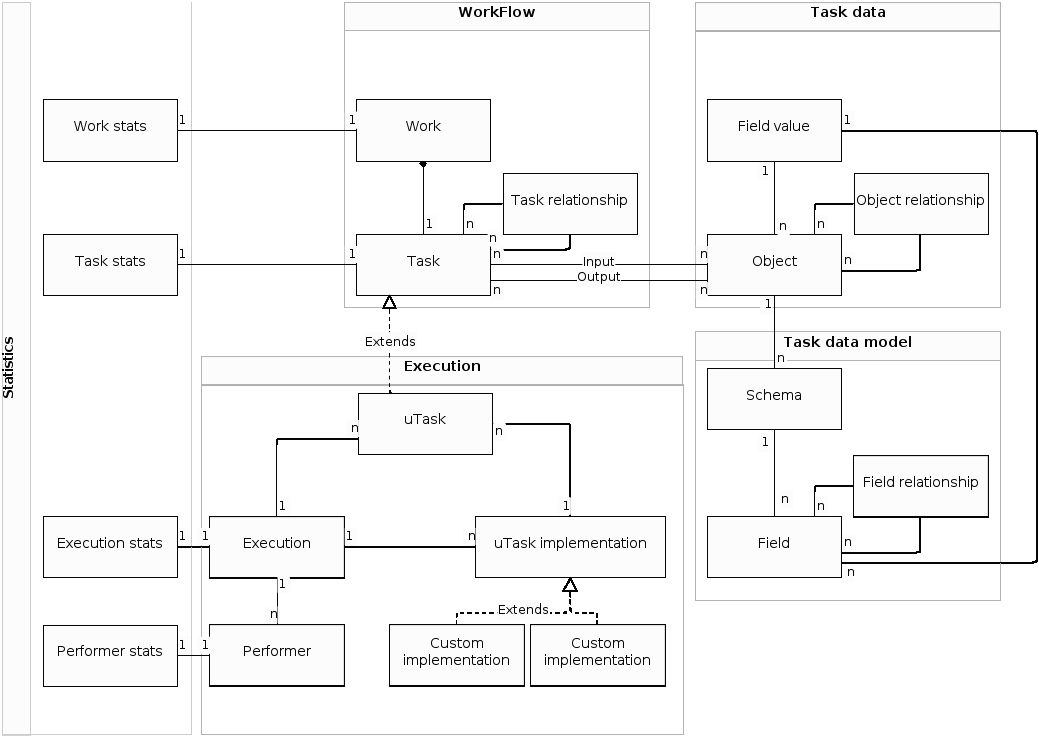
\includegraphics[width=\columnwidth]{DataModel}
    \caption{Overall Data Model schema, with logical subdivision.}
    \label{fig:data-model}
\end{figure}
\begin{figure}[htb]
    \centering
    
\includegraphics[width=0.75\columnwidth]{ConceptualModel}
    \caption{Conceptual organization of Work, Task and \utask{}.}
    \label{fig:conceptual-model}
\end{figure}

\subsection{WorkFlow}
The WorkFlow embodies all the data associated to the \emph{flow} of Task
that need to be executed in order to complete a set of Tasks. The tasks can belong
to different archetypes (e.g. Human, Automatic) and have their own set of assigned
objects. The \emph{Workflow} is composed of:
\begin{description}
    \item[The Work:] is the abstract representation of a set of Tasks related
    to each other.
    \item[The Flow:] describes how the Tasks, belonging to a Work, are related
    to each other, also defining the type (e.g. dependency, parallel) of relation
    between such Tasks. 
    \item[The Task:] is the representation of a general activity that can be
    performed by the framework.
\end{description}

\subsubsection{The Work}\label{data:work}
The \emph{Work} represents a set of related Tasks finalized to the execution of
some kind of data manipulation or analysis on a set of input Objects. The
result of the execution produces output Objects described by a Schema. The Work
is defined by:
\begin{itemize}
    \item A \textbf{Name} that identifies the Work.

    \item \textbf{Constraints} used to bind some aspects of the Work or to make
    decision for giving less or more priority to this work with respect to the
    others. Example of constraints are: Due date, Performer skills, Max execution
    time, etc.

    \item \textbf{Input} data, defined by a \emph{Schema} and the associated
    Objects. To keep the model as general as possible no assumptions are made on
    the \emph{Schema} type (relational, graph, etc.).
    \item \textbf{Output} data, defined as an extension of the input schema
    (sharing the same schema type).

    \item A set of \textbf{Task} composing the Work. Their orchestration is made
    at design time, by specifying a \emph{Flow}.
\end{itemize}

\subsubsection{The Task}\label{data:task}
The Task is the central unit of computation. It represents a single activity
focusing on a particular action. The activity must not be an atomic operation,
like in an algorithm a single function call, but it should be focused on a
single purpose. For example tagging an image can be considered as a single Task.
Otherwise tagging and validating an image should be divided in two separated
tasks if possible. The flexibility of the framework allows the creation of any
type of Task, the previous statement is only an advice to better separate
different activities into different Task. As we mentioned our system can
seamlessly handle complex Task involving multiple activities, such as whole
\ac{GWAP} game into a single Task. A Task is characterized by:
\begin{itemize}
    \item A \textbf{Name} that identifies the Task.

    \item \textbf{Input} data, defined by a \emph{Schema} and the associated
    Objects. To keep the model as general as possible no assumptions are made on
    the \emph{Schema} type (relational, graph, etc.). Usually the Schema
    is a projection of the Schema of a Work. Like the Schema the input Objects
    usually are a selection of the Work input Objects.
    \item \textbf{Output} data, defined as an extension of the input schema
    (sharing the same schema type).

    \item A Task \textbf{type}\footnote{An assumption is made to make the list fit
    all the possible abstract tasks our framework is able to handle.}
    defining, at abstract level, what kind of data manipulation will be performed
    by a Task. These categorizations are taken from \cite{paperboz}, here there are a
    few:
        \begin{itemize}
            \item Like
            \item Order
            \item Classify
            \item Add
            \item \omissis
        \end{itemize}
    \noindent Each Task type is defined by:
        \begin{itemize}
            \item I/O relationship, defining, at abstract level, how the Task
            transforms the data and the schema.
            \item A default implementation.
        \end{itemize}

    \item A \textbf{Status} encoding the current state of the Task. A Task, can
    have only one of the following statuses at point of its lifecycle:
        \begin{itemize}
            \item \emph{Planning-Input}: the Task has been created, has a
            \emph{Schema} and \emph{Object data} associated and a defined Task
            \emph{type}.

            \item \emph{Planning-\utask{}}: a set of \utask{} has been associated
            to the Task.
            
            \item \emph{Planning-Assignment}: a set of \emph{Performers} has
            been selected to execute the \utask{}.
            
            \item \emph{Wait}: Task planned, \utask{} ready for execution.
            
            \item \emph{Running}: \utask{}s are running.
            
            \item \emph{Ended}: all the \utask{}s have completed their execution.
        \end{itemize}
    
    \item A set of \textbf{Subscriber}s able to receive updates on the Task
    execution. The Subscribers are declared during the Task creation step and the
    updates that they will receive are about change on the Status of the Task.

    \item A set of \textbf{Execution constraints} used for prioritizing the Task
    among others or to modify the standard behavior of the Task. The constraints
    that can be used are the same defined for the Work in \ref{data:work}.

    \item \textbf{Configuration data} are application specific data used to
    configure the behavior of the Task once it is executing. For instance
    we can store here the classes for a classify Task type.

    \item \textbf{\utask{}}s are the instances of a Task assigned to one or more
    Performers.

    \item An \textbf{Aggregation} function, in charge of collecting the \utask{}s
    results and generate the Task output.
    
    \item \textbf{\utask{} planning} strategy, in charge of defining how many
    \utask{}s create for a given Task and associate the right portion of input
    objects to each \utask{}. For example total disjunction, redundancy, partial
    overlap, etc.
    
    \item \textbf{Performer assignment} strategy able to assign \emph{Performers}
    to \utask{}s. Some strategies can be: manual, random, most reliable, etc.

    \item \textbf{\utask{} implementation} strategy in charge of routing the
    correct \utask{} implementation for each \utask{} execution. The routing
    can be \emph{fixed} for everyone, can be done according to the
    \emph{user-agent} (e.g. Browser) or other conditions.

    \item A \textbf{Task planning} which embodies the functionalities of
    \emph{\utask{} planning} strategy, \emph{Performer assignment} strategy and
    \emph{\utask{} implementation} strategy and whose purpose is to decide the 
    logic behind the invocation of those strategies.

    \item A \textbf{Task control} strategy is able to control the status of the
    Task and if needed perform corrective actions.

    \item An \textbf{Emission policy} specifying which \emph{Subscriber} needs to
    be notified of a Task change in \emph{Status}.
\end{itemize}


The \textbf{relationships} that may exist between Tasks are materialized into the
\emph{Task Relationship} object. This object contains all the information related
to the flow of the task execution during the execution of a Work. An example of
a Task relation can be the validation of the results obtained by an Automatic
computation task previously performed. In this case the relation is the simple
sequence.

In a flow we can use \emph{Control Structures} and \emph{Variables}. The
\emph{variables} are included in the flow to control the behavior of the Work
and can be modified by some conditions upon Task execution. For instance after
obtaining Task results we found that they are under a certain threshold then we
can set a variable to match this problem.

The \emph{Control Structures} are common to all the Workflow managers and 
control how the Tasks are executed:
\begin{description}
     \item[Sequence:] represents the normal flow of an application where one
     operation is executed after the previous is completed.
     \item[Choice:] gives the possibility to made choice according to one, or
     more, \emph{Variables}.
     \item[Loop:] Allows to execute some steps multiple times, according to a
     predefined value or a \emph{Variable}.
     \item[Parallel:] the steps of the flow are not executed in \emph{Sequence},
     allowing the parallelization of some steps.
 \end{description} 









\subsection{Task Data Model}\label{data:model}
The Task Data Model contains all the information about the Task metamodel. The
metamodel is organized in Fields and the Fields are grouped into a Schema. This
data structure resembles the standard DBMS schema organization, where we have
a Schema defined as a collection of Fields with possible relationship between
them. The Task Data Model is composed by
\begin{description}
    \item[The Schema:] is the abstract representation of a table structure.
    \item[The Field:] contains all the information of the field type and
    relationships.
\end{description}


\subsubsection{The Schema}
The Schema is used as a container of Fields that composes the metamodel of the
Task data. The Schema is defined by:
\begin{itemize}
    \item A \textbf{Name}

    \item A \textbf{list of Fields} defining the structure of the Task data.
\end{itemize}

The Schema is in \textbf{relation} with the actual data instances of the Task,
called Objects, and the Fields it is composed of.


\subsubsection{The Field}
The Field contains information on the type of the data it contains and information
on the relation between two, or more, Fields (like the type of dependency).
The Field is composed by:
\begin{itemize}
    \item A \textbf{Name} that identifies the Field.
    
    \item A \textbf{type} defining the type of the data that this field contains,
    for instance \code{string}, \code{number}, etc.

    \item A set \textbf{related fields}. The relationship between the fields
    is defined by the \emph{relation} attribute.
    
    \item A \textbf{relation} that specifies which type of relationship occurs
    among the \emph{related fields}.

    \item The \textbf{list of field values} representing the data contained within
    this field in the Object structure.
\end{itemize}

The \textbf{relationship}s existing between the Field are materialized using the
\emph{Field Relationship} table. Here we have all the information of the fields
involved and on the type of the relationship (e.g. derivate of, copy of, calculated
etc.). Each field has also a relationship with the corresponding instances
in the \emph{Field Values} table.








\subsection{Task Data}
The Task Data contains the actual data instance for each Task. The data
are subdivided into \emph{Field Values} and \emph{Objects}. This division is made
to mirror the structure presented in \ref{data:model}. The Objects represent
the "tuple" of the table, while the Field Values contain the atomic information
of a Field within a Tuple. This structure allows the direct access to Field
Values without the need of parsing the whole Object element. As mentioned the
Task Data is composed of:
\begin{description}
    \item[The Object:] a Task data instance, represented by a set of Field Values.
    \item[The Field Value:] represents the instance of a Field. As the Fields
    they can be related to each other.
\end{description}


\subsubsection{The Object}
The Object represents the Task data instances. They are composed of a set of
Field Values that, joined together, form the Object. The object itself is
composed by:
\begin{itemize}
    \item A \textbf{Name}.
    \item A \textbf{list of Field Value}s data.
\end{itemize}

Objects can have \textbf{relationships} among them. These relationships are
materialized into the \emph{Object Relationship} entity. This object contains
the needed information used to identify a set of Objects belonging to a
particular Task.



\subsubsection{The Field Value}
The Field Value contains the actual data of a Field. Since this object is used
to represent any kind of data, it must be able to handle different types of
information (e.g. \code{string}, \code{BLOB}, \code{number}, \code{date}, etc.).
The Task Field is composed by:
\begin{itemize}
    \item The field \textbf{Value}.
    \item A \textbf{related Object} used to identify to which Object this Field
    Value belongs to.
    \item The \textbf{Field} to which data belongs.
\end{itemize}

The Field Value has \textbf{relationships} with the Object to which it belongs
and with the Field that defines the general type of the Field Value.








\subsection{Task Execution}
The Task Execution is used to collect information on the Task execution. Since
a Task must be distributed to multiple nodes\footnote{We use the broad term node
to identify both the user and the device on which the Task must be executed.} the
Task must be splitted in \utask{}. Then we need to know what user is performing
such \utask{}, and, based on the device used, we can have multiple implementations
of the same \utask{}. All these information are subdivided into:
\begin{description}
    \item[The \utask{}:] is a subclass of the Task. The \utask{} is a portion
    of the Task executed by the end-user.
    \item[The \utask{} Implementation:] represents the real implementation
    of the \utask{}.
    \item[The Performer:] is the Human being in charge of the execution of the
    Task.
    \item[The Execution:] represents a bridge object connecting the \utask{},
    the \utask{} Implementation and the Performer to identify the execution of a
    \utask{} using a \utask{} implementation by a particular user.
\end{description}


\subsubsection{\utask{}}
Since the same Task must be distributed to many users there is the need of a
further subdivision of a Task into "atomic" activities (see
\autoref{fig:conceptual-model}).
The \utask{} is a subclass of the Task that represents this subdivision. As
a subclass it inherits all the information of the data and the schema from the
parent Task. Usually \utask{}s have associated only a portion of the parent
Task data objects. The \utask{} is defined by:
\begin{itemize}
    \item A \textbf{Name}.
    
    \item A set of \textbf{Execution constraints}, similar to the ones defined
    in \ref{data:work}. The difference is that these constraints bind the
    execution "client side". This means that with these we can control the
    computational load on the user machine according to some policy (like
    user preferences, device capabilities, etc).
    
    \item \textbf{Input} data, as a subset of the Task input Objects.
    \item \textbf{Output} data, with the same schema as the related Task output
    Objects.
    
    \item A \textbf{list of Properties}, defined as name-value pairs, having
    domain specific meaning.
\end{itemize}

The \utask{} is in \textbf{relationship} with its \utask{} implementations. This
relation is useful when choosing a suitable implementation to execute on a
particular device.



\subsubsection{\utask{} implementation}
The \utask{} Implementation represents the application logic and presentation
delivered to a user to perform a Task. The Task has a default implementation
and the other implementations can be supplied to customize the Task execution.
Each \utask{} implementation is in \textbf{relation} with the corresponding
\utask{}.




\subsubsection{Performer}
The Performer is an object used to characterize a human being in the Data Model.
The user is characterized with properties that defines his/her skills on a
certain field (like music, style, etc.) and some other attributes used for
profiling. The Performer object is defined by
\begin{itemize}
    \item A \textbf{Name}.
    \item \textbf{Demographic} information.
    \item \textbf{Performance} information.
    \item \textbf{Trustworthiness}.
    \item \textbf{Social properties}.
\end{itemize}



\subsubsection{The Execution}
The Execution is a bridge object that joins together \utask{}, \utask{}
implementation and performer. This object represents a single instance execution
of a Task by a user. Using this object we can identify cheaters or reward good
Performers, or using it as a timeline we can see how the Performers respond to
the Task and change it accordingly. An Execution object is defined by:
\begin{itemize}
    \item A \textbf{Status} that identifies the current status of a \utask{}
    implementation. The available statuses are:
    \begin{itemize}
        \item \emph{running}
        \item \emph{suspended}
        \item \emph{idle}
        \item \emph{ended}
    \end{itemize}

    \item A \textbf{set of Execution data}.
\end{itemize}

Since it is a bridge object the Execution has \textbf{relationship}s with 
\utask{}, \utask{} implementation and the Performer. These relationships
identify the Execution itself.



\subsection{Statistics}
This Statistics model contains all the statistics and data related to the profiling
of a Task. These data can be used by other components, such as the Task controller
to take decision during the flow of a Task. The Statistics are about \emph{Work},
\emph{Task}, \emph{\utask{}}, \emph{Performer}, etc. The data contained in these
objects are:
\begin{itemize}
    \item \textbf{Creation date}.
    \item \textbf{Total execution time}.
    \item \textbf{Average number of \emph{Performer}s per hour}.
    \item \textbf{Last execution}.
    \item Etc.
\end{itemize}
